%%%%%%%%%%%%%%%%%%%%%%%%%%%%%%%%%%%%%%%%%%%%%%%%%%%%%%%%%%%%%%%%%%%%%%%%%%%%%%%%%%
\begin{frame}[fragile]\frametitle{}
\begin{center}
{\Large Small Talk}

{\tiny (Ref: https://rasa.com/docs/rasa/dialogue-elements/small-talk/ )}
\end{center}
\end{frame}

%%%%%%%%%%%%%%%%%%%%%%%%%%%%%%%%%%%%%%%%%%%%%%%%%%%%%%%%%%%
 \begin{frame}[fragile]\frametitle{What is SmallTalk?}
\begin{itemize}
\item The back-and-forth that makes conversations natural
\item But doesn’t directly relate to the user’s goal.
\item Includes greetings, acknowledgments, reactions, and off-topic chitchat.
\end{itemize}
\end{frame}

%%%%%%%%%%%%%%%%%%%%%%%%%%%%%%%%%%%%%%%%%%%%%%%%%%%%%%%%%%%
 \begin{frame}[fragile]\frametitle{Greetings}
\begin{itemize}
\item Almost every chatbot should have these
\item Use ``MappingPolicy'' if you want same responses for each such intent via triggers
\end{itemize}

\begin{lstlisting}
intents:
  - greet: {triggers: utter_greet}
  - goodbye: {triggers: utter_goodbye}
\end{lstlisting}

Make sure the mapping policy is present in your config.yml

\begin{lstlisting}
policies:
  - name: "MappingPolicy"
  ...
\end{lstlisting}

\end{frame}

%%%%%%%%%%%%%%%%%%%%%%%%%%%%%%%%%%%%%%%%%%%%%%%%%%%%%%%%%%%
 \begin{frame}[fragile]\frametitle{Greetings}
\begin{itemize}
\item If you want to implement less rigid behaviour, use regular stories instead of the mapping policy
\item Say, if you want to send a special response if the user says goodbye immediately after saying hello, remove the triggers metadata from the domain file, and include relevant stories in your training data
\end{itemize}

\begin{lstlisting}
* greet
  - utter_greet
* goodbye
  - utter_ask_why_leaving
\end{lstlisting}

\end{frame}

%%%%%%%%%%%%%%%%%%%%%%%%%%%%%%%%%%%%%%%%%%%%%%%%%%%%%%%%%%%
 \begin{frame}[fragile]\frametitle{Acknowledgments}
\begin{itemize}
\item At certain point in time, user will expect an acknowledgment.
\item It reassures the user that their message has been received.
\item First, you need NLU data for reactions and acknowledgments:
\begin{lstlisting}
## intent:acknowledge
- ok
- got it
- understood
- k

## intent:opinion+positive
- nice!
- excellent
- that's awesome

## intent:opinion+negative
- ugh
- that sucks
- woah! that's [expensive](price)
\end{lstlisting}
\end{itemize}
\end{frame}

%%%%%%%%%%%%%%%%%%%%%%%%%%%%%%%%%%%%%%%%%%%%%%%%%%%%%%%%%%%
 \begin{frame}[fragile]\frametitle{Acknowledgements}
\begin{itemize}
\item And then you need training stories to teach Rasa how to respond:
\begin{lstlisting}
## price reaction
* opinion+negative{"price": "expensive"}
  - utter_good_value
  - utter_ask_continue

## simple acknowledgement
* opinion+positive
  - utter_positive_feedback_reaction
\end{lstlisting}
\end{itemize}
\end{frame}

%%%%%%%%%%%%%%%%%%%%%%%%%%%%%%%%%%%%%%%%%%%%%%%%%%%%%%%%%%%
 \begin{frame}[fragile]\frametitle{Chitchat}
\begin{itemize}
\item If your chatbot receives unexpected or unprompted input, its called as Chitchat
\item Typically its not possible to react to it in coherent manner, but we can just acknowledge it.
\end{itemize}

\begin{center}
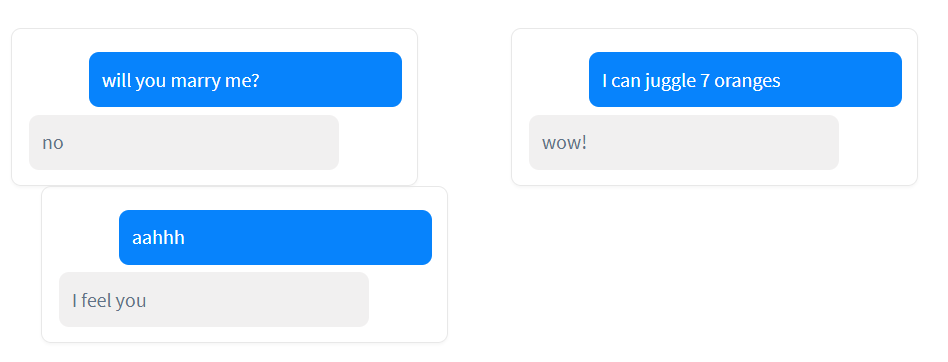
\includegraphics[width=0.8\linewidth,keepaspectratio]{rasa37}
\end{center}
\end{frame}

%%%%%%%%%%%%%%%%%%%%%%%%%%%%%%%%%%%%%%%%%%%%%%%%%%%%%%%%%%%
 \begin{frame}[fragile]\frametitle{Insults}
\begin{itemize}
\item Sometimes the user may abuse the chatbot.
\item You should acknowledge the nature of their comment and respond in a way that reflects your assistant’s persona. 
\item Responding with a joke can encourage users to continue sending abuse, so consider your responses carefully
\item The simplest approach is to create a single insult intent and use the mapping policy to respond to it:
\end{itemize}

\begin{center}
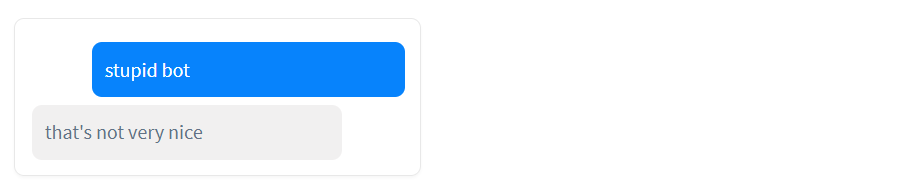
\includegraphics[width=0.8\linewidth,keepaspectratio]{rasa38}
\end{center}
\end{frame}

%%%%%%%%%%%%%%%%%%%%%%%%%%%%%%%%%%%%%%%%%%%%%%%%%%%%%%%%%%%
 \begin{frame}[fragile]\frametitle{Insults}
\begin{itemize}
\item In your domain file:
\begin{lstlisting}
intents:
  - insult: {triggers: utter_respond_insult}
\end{lstlisting}
\item And in your configuration file:
\begin{lstlisting}
policies:
  - name: "MappingPolicy"
  ...
\end{lstlisting}
\end{itemize}

\end{frame}